\documentclass{article}

% these packages let you do math
\usepackage{amsmath}
\usepackage{amssymb}

% we need these packages for fancy R tables
\usepackage{booktabs}
\usepackage{float}
\usepackage{colortbl}
\usepackage{xcolor}

% these packages play with the spacing/margins of the document. Uncomment the commands on lines 16 and 17 to see what they do.
\usepackage{a4wide}
\usepackage{setspace}
\usepackage{geometry}
\usepackage{parskip}
%\doublespacing
%\geometry{margin=1.5in}

% this package helps us with including images. Setting the graphics path makes it easier to refer to things in the \includegraphics command.
\usepackage{graphicx}
\graphicspath{ {C:/Users/jinki/Documents/my-first-rproject/GitHub/figures/} }

% make some hyperlinks using the \href command
\usepackage{hyperref}
\hypersetup{
    colorlinks=true,
    linkcolor=black,
    urlcolor=blue
}

% set the author, title, and date of the document. \maketitle adds it to the document.
\author{Kiyea Jin}
\title{Incarceration Status by Gender and Race}
\date{2/18/2022}

\begin{document}
\maketitle

\section{Introduction}

Youth crime has been one of the most crucial social issues; much efforts have been made to reduce crime rate of youth. The debate about what effects youth crime, both in an academic context as well as the government's policies, has intensified. I contribute to the debate by figuring out patterns in incarceration status of youth by race and gender, especially focusing on the year 2002. 


\section{Data}

This paper estimates the model using data from National Longitudinal Survey of Youth 1997 (NLSY97), which is a program of the U.S. Bureau of Labor Statistics.\footnote{The data is from the \href{https://www.nlsinfo.org/investigator/pages/search}{NLS Investigator}.} The incarceration event history arrays consist of monthly variables that document the number of incarcerations in each month starting at the respondent's 12th birthday. It starts in January 1992 and ends with the most recent publicly available interview date.

 
\begin{figure}[H]
    \begin{center}
        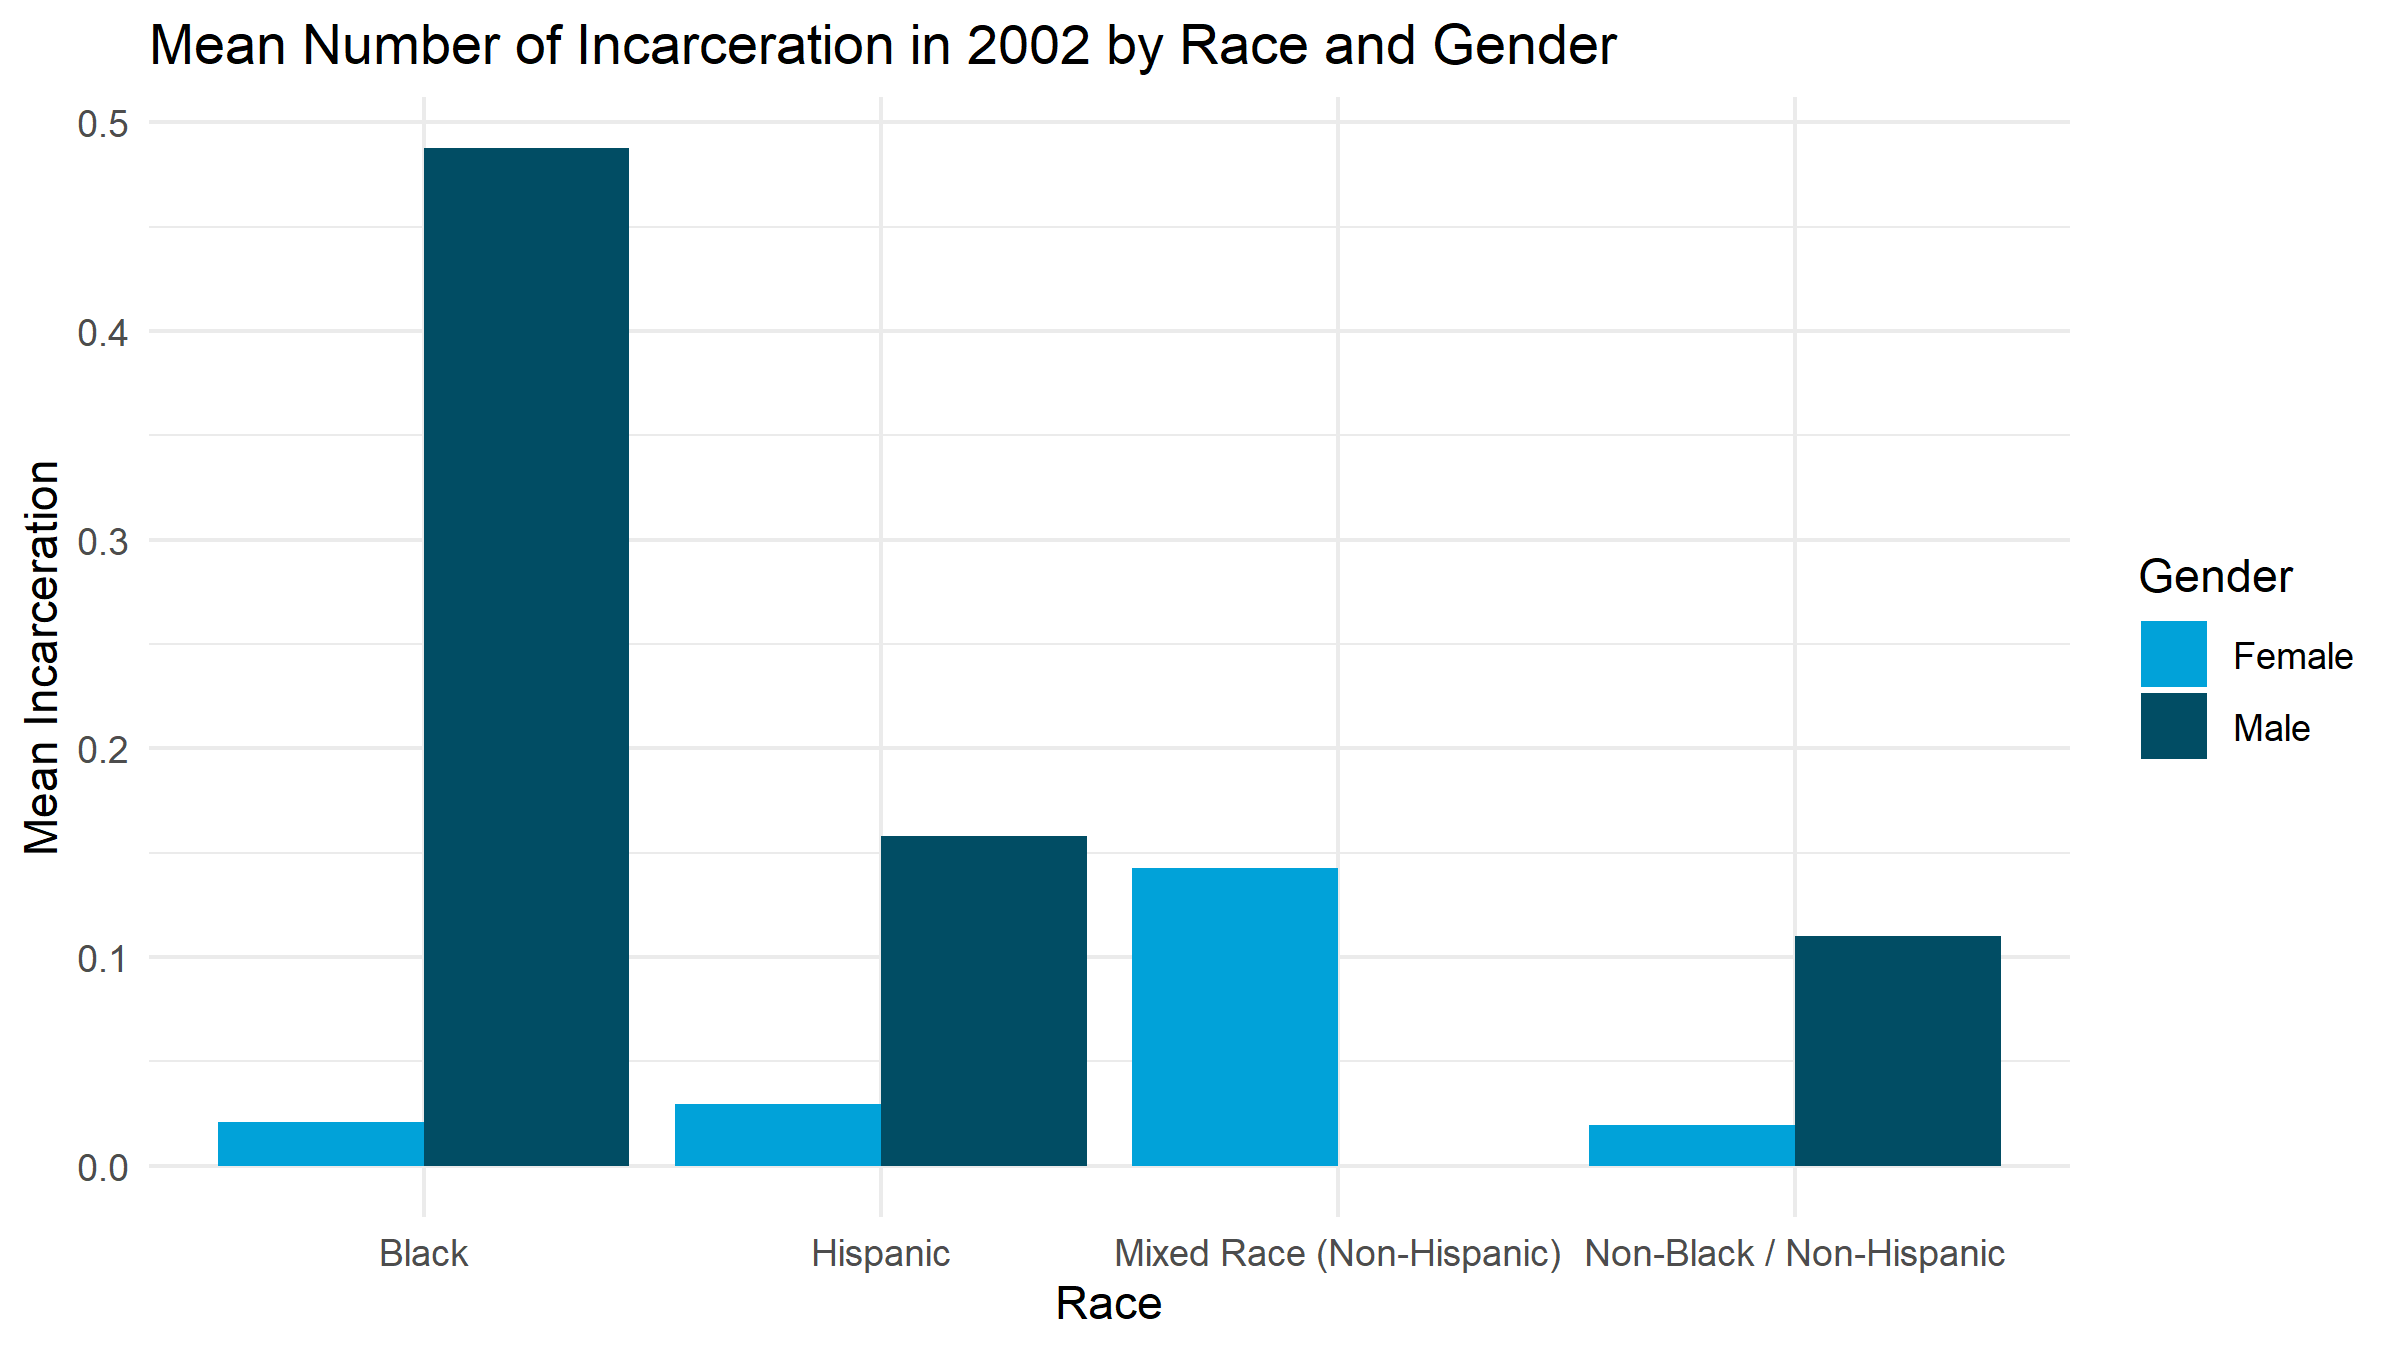
\includegraphics[width=0.7\textwidth]{incarceration_by_racegender}
    \end{center}
    \caption{Mean Number of Incarceration in 2002 by Race and Gender}
    \label{fig:graph}
\end{figure}


\newpage

\texttt{Figure 1} provides evidence for the fact that I am interested in. The mean number of incarceration seems to vary significantly by race and gender. As shown below, the mean number of  incarceration of Black is significantly high. Also, it shows that the mean number of incarceration of male is higher than that of woman excluding the case of mixed race (Non-Hispanic).  

\vspace{2cm}
\section{Results}

\texttt{Table 1} below shows the exact numbers. As we saw from \texttt{Figure 1}, there exist discernible patterns in incarceration status by race and gender. When we see the \texttt{Table 1} vertically, the value are high in Black, which is followed by Hispanic. On the other hand, the value of male is always higher than that of female except Mixed Race case.

\begin{table}[H]

\caption{\label{tab:tab:summarystats}Mean incarceration in 2002 by Race and Gender}
\centering
\begin{tabular}[t]{lrrrr}
\toprule
Gender & Black & Hispanic & Mixed Race Non Hispanic & Non Black Non Hispanic\\
\midrule
\cellcolor{gray!6}{Female} & \cellcolor{gray!6}{0.0211268} & \cellcolor{gray!6}{0.0298013} & \cellcolor{gray!6}{0.1428571} & \cellcolor{gray!6}{0.0193192}\\
Male & 0.4876712 & 0.1579509 & 0.0000000 & 0.1099476\\
\bottomrule
\end{tabular}
\end{table}


\vspace{1cm}
To examine if race and gender are statistically significant in accounting for incarceration status of youth, we estimate the regression model including dummy variables indicating each race and gender. Note that the omitted category is Black Females. The \texttt{equation} is as follows:

\vspace{0.5cm}
\begin{equation*}
    incarceration = \beta_0 + \beta_1Male + \beta_2Non-Black/Non-Hispanic + \beta_3Mixed Race + \beta_4Hispanic + \varepsilon
\end{equation*}
\vspace{0.5cm}

The results for all the estimated parameters are presented in \texttt{Table 2}. The results confirm all the findings in the previous analysis; it shows that race and gender explain incarceration status well as F statistic is statistically significant in 1\% significance level. In specific, all the estimated coefficients of race variables are negative; the other races - such as Hispanic, Mixed Race, or Non-Black and Non-Hispanic - have statistically significant effect on incarceration status, reducing the mean number of incarceration compared to Black. On the other hand, the estimated coefficient of Male variable is statistically significant in 1\% significance level and has a positive sign; it implies that males are more likely to be in incarceration than females are.


% Table created by stargazer v.5.2.2 by Marek Hlavac, Harvard University. E-mail: hlavac at fas.harvard.edu
% Date and time: Wed, Feb 16, 2022 - 4:16:28 PM
\begin{table}[!htbp] \centering 
  \caption{Regression Output. Omitted category is Black Females.} 
  \label{tab:regression} 
\begin{tabular}{@{\extracolsep{5pt}}lc} 
\\[-1.8ex]\hline 
\hline \\[-1.8ex] 
 & \multicolumn{1}{c}{\textit{Dependent variable:}} \\ 
\cline{2-2} 
\\[-1.8ex] & Incarceration in 2002 \\ 
\hline \\[-1.8ex] 
 Hispanic & $-$0.159$^{***}$ \\ 
  & (0.038) \\ 
  & \\ 
 Mixed Race (Non-Hispanic) & $-$0.174$^{**}$ \\ 
  & (0.083) \\ 
  & \\ 
 Non-Black / Non-Hispanic & $-$0.189$^{***}$ \\ 
  & (0.035) \\ 
  & \\ 
 Male & 0.194$^{***}$ \\ 
  & (0.022) \\ 
  & \\ 
 Constant & 0.155$^{***}$ \\ 
  & (0.026) \\ 
  & \\ 
\hline \\[-1.8ex] 
Observations & 8,621 \\ 
R$^{2}$ & 0.015 \\ 
Adjusted R$^{2}$ & 0.014 \\ 
Residual Std. Error & 1.019 (df = 8616) \\ 
F Statistic & 32.033$^{***}$ (df = 4; 8616) \\ 
\hline 
\hline \\[-1.8ex] 
\textit{Note:}  & \multicolumn{1}{r}{$^{*}$p$<$0.1; $^{**}$p$<$0.05; $^{***}$p$<$0.01} \\ 
\end{tabular} 
\end{table} 




\end{document}
